\section{Техническое задание}
\subsection{Основание для разработки}

Основанием для разработки программного продукта служит задание курсовой работы «Растровый графический редактор» по дисциплине «Языки объектно-ориентированного программирования».

\subsection{Цель и назначение разработки}

Основной задачей курсовой работы является разработка программного продукта для создания и редактирования графических изображений.

Задачами данной разработки являются:
\begin{itemize}
\item разработка архитектуры приложения;
\item реализация возможности создавать файл с графическим изображением;
\item разработка интерфейса приложения;
\item реализация возможности открывать, редактировать и сохранять файл с графическим изображением;
\item реализация возможности менять размер, создаваемого полотна;
\item реализация возможности наблюдать изменения, происходящие на экране, которые вызваны действиями пользователя;
\item реализация возможности изменять параметры кисти: размер, цвет;
\end{itemize}

\subsection{Требования пользователя к интерфейсу приложения}

Приложение должен включать в себя:
\begin{itemize}
	\item начальное окно с параметрами создаваемого холста;
	\item панель для работы с файлом: сохранение, удаление, открытие другого файла;
	\item панель для работы с инструментами: кисть, ластик.
	\item панель для работы с параметрами инструмента: цветом и размером;
\end{itemize}

Композиция шаблона приложения представлена на рисунке ~\ref{shablon:image}.

\begin{figure}[ht]
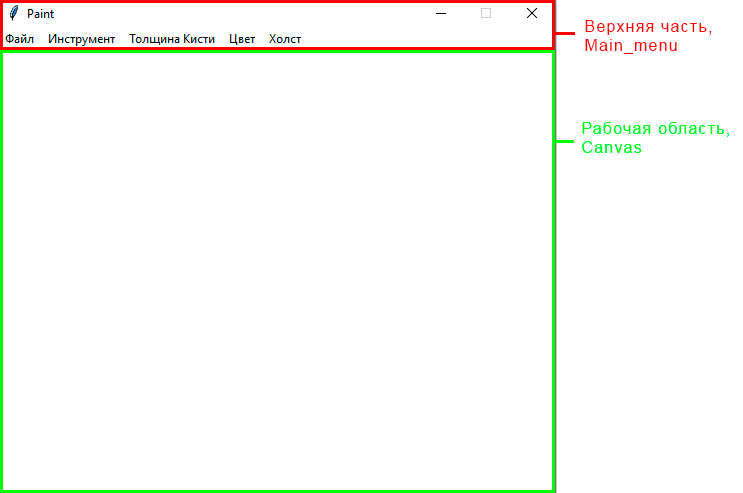
\includegraphics[width=1\linewidth]{shablon}
\caption{Композиция шаблона приложения}
\label{shablon:image}
\end{figure}
%\vspace{-\figureaboveskip} % двойной отступ не нужен (можно использовать, если раздел заканчивается картинкой)

\subsection{Моделирование вариантов использования}

Для разрабатываемого приложения была реализована модель, которая обеспечивает наглядное представление вариантов использования приложения.

Она помогает в физической разработке и детальном анализе взаимосвязей объектов. При построении диаграммы вариантов использования применяется унифицированный язык визуального моделирования UML.

Диаграмма вариантов описывает функциональное назначение разрабатываемой системы. То есть это то, что система будет непосредственно делать в процессе своего функционирования. Она является исходным концептуальным представлением системы в процессе ее проектирования и разработки. Проектируемая система представляется в виде ряда прецедентов, предоставляемых системой актерам или сущностям, которые взаимодействуют с системой. Актером или действующим лицом является сущность, взаимодействующая с системой извне (например, человек, техническое устройство). Прецедент служит для описания набора действий, которые система предоставляет актеру.

На основании анализа предметной области в программе должны быть реализованы следующие прецеденты:
\subsubsection{Первый запуск}

При первом запуске программы пользователь должен выбрать ширину и высоту будущего изображения в начальном окне. Если введенные данные корректны, то пользователь получает доступ к основному окну.

\subsubsection{Сохранение}

При нажатии пользователем кнопки «Сохранить», открывается диалоговое окно, в котором пользователь должен выбрать имя и путь к изображению.

\subsubsection{Открытие}

При нажатии пользователем кнопки «Открыть», открывается диалоговое окно, в котором пользователь должен выбрать уже существующее изображение для редактирования.

\subsubsection{Рисование}

При нажатии в рабочую зону левой кнопкой мыши, появляется точка определенного радиуса. Если пользователь будет удерживать левую кнопку мыши, то точки, появляющиеся в рабочей зоне, начнут соединяться, образуя линии.

\subsubsection{Смена размера}

При выборе любого пункта в разделе «Толщина кисти», пользователь изменяет радиус создаваемой точки из прецедента «Рисование».

\subsubsection{Смена цвета}

При выборе любого пункта в разделе «Цвет», пользователь изменяет цвет создаваемой точки из прецедента «Рисование».

\subsubsection{Цвет холста}

При выборе пункта «Цвет холста», пользователь изменяет цвет всей рабочей зоны на выбранный.

\subsubsection{Очистка холста}

При выборе пункта «Очистка холста», пользователь изменяет цвет всей рабочей зоны на белый.

\subsection{Требования к оформлению документации}

Разработка программной документации и программного изделия должна производиться согласно ГОСТ 19.102-77 и ГОСТ 34.601-90. Единая система программной документации.
